%% bare_conf_compsoc.tex
%% V1.4b
%% 2015/08/26
%% by Michael Shell
%% See:
%% http://www.michaelshell.org/
%% for current contact information.
%%
%% This is a skeleton file demonstrating the use of IEEEtran.cls
%% (requires IEEEtran.cls version 1.8b or later) with an IEEE Computer
%% Society conference paper.
%%
%% Support sites:
%% http://www.michaelshell.org/tex/ieeetran/
%% http://www.ctan.org/pkg/ieeetran
%% and
%% http://www.ieee.org/

%%*************************************************************************
%% Legal Notice:
%% This code is offered as-is without any warranty either expressed or
%% implied; without even the implied warranty of MERCHANTABILITY or
%% FITNESS FOR A PARTICULAR PURPOSE! 
%% User assumes all risk.
%% In no event shall the IEEE or any contributor to this code be liable for
%% any damages or losses, including, but not limited to, incidental,
%% consequential, or any other damages, resulting from the use or misuse
%% of any information contained here.
%%
%% All comments are the opinions of their respective authors and are not
%% necessarily endorsed by the IEEE.
%%
%% This work is distributed under the LaTeX Project Public License (LPPL)
%% ( http://www.latex-project.org/ ) version 1.3, and may be freely used,
%% distributed and modified. A copy of the LPPL, version 1.3, is included
%% in the base LaTeX documentation of all distributions of LaTeX released
%% 2003/12/01 or later.
%% Retain all contribution notices and credits.
%% ** Modified files should be clearly indicated as such, including  **
%% ** renaming them and changing author support contact information. **
%%*************************************************************************


% *** Authors should verify (and, if needed, correct) their LaTeX system  ***
% *** with the testflow diagnostic prior to trusting their LaTeX platform ***
% *** with production work. The IEEE's font choices and paper sizes can   ***
% *** trigger bugs that do not appear when using other class files.       ***                          ***
% The testflow support page is at:
% http://www.michaelshell.org/tex/testflow/



\documentclass[conference,compsoc]{IEEEtran}
% Some/most Computer Society conferences require the compsoc mode option,
% but others may want the standard conference format.
%
% If IEEEtran.cls has not been installed into the LaTeX system files,
% manually specify the path to it like:
% \documentclass[conference,compsoc]{../sty/IEEEtran}





% Some very useful LaTeX packages include:
% (uncomment the ones you want to load)


% *** MISC UTILITY PACKAGES ***
%
%\usepackage{ifpdf}
% Heiko Oberdiek's ifpdf.sty is very useful if you need conditional
% compilation based on whether the output is pdf or dvi.
% usage:
% \ifpdf
%   % pdf code
% \else
%   % dvi code
% \fi
% The latest version of ifpdf.sty can be obtained from:
% http://www.ctan.org/pkg/ifpdf
% Also, note that IEEEtran.cls V1.7 and later provides a builtin
% \ifCLASSINFOpdf conditional that works the same way.
% When switching from latex to pdflatex and vice-versa, the compiler may
% have to be run twice to clear warning/error messages.


% \usepackage[utf8]{inputenc}
% \usepackage{natbib}
\usepackage{graphicx}

\usepackage{hyperref}
\usepackage[inline]{enumitem}
% \usepackage{cite}



% *** CITATION PACKAGES ***
%
% \ifCLASSOPTIONcompsoc
  % IEEE Computer Society needs nocompress option
  % requires cite.sty v4.0 or later (November 2003)
%   \usepackage[nocompress]{cite}
% \else
  % normal IEEE
  \usepackage{cite}
% \fi
% cite.sty was written by Donald Arseneau
% V1.6 and later of IEEEtran pre-defines the format of the cite.sty package
% \cite{} output to follow that of the IEEE. Loading the cite package will
% result in citation numbers being automatically sorted and properly
% "compressed/ranged". e.g., [1], [9], [2], [7], [5], [6] without using
% cite.sty will become [1], [2], [5]--[7], [9] using cite.sty. cite.sty's
% \cite will automatically add leading space, if needed. Use cite.sty's
% noadjust option (cite.sty V3.8 and later) if you want to turn this off
% such as if a citation ever needs to be enclosed in parenthesis.
% cite.sty is already installed on most LaTeX systems. Be sure and use
% version 5.0 (2009-03-20) and later if using hyperref.sty.
% The latest version can be obtained at:
% http://www.ctan.org/pkg/cite
% The documentation is contained in the cite.sty file itself.
%
% Note that some packages require special options to format as the Computer
% Society requires. In particular, Computer Society  papers do not use
% compressed citation ranges as is done in typical IEEE papers
% (e.g., [1]-[4]). Instead, they list every citation separately in order
% (e.g., [1], [2], [3], [4]). To get the latter we need to load the cite
% package with the nocompress option which is supported by cite.sty v4.0
% and later.





% *** GRAPHICS RELATED PACKAGES ***
%
\ifCLASSINFOpdf
  % \usepackage[pdftex]{graphicx}
  % declare the path(s) where your graphic files are
  % \graphicspath{{../pdf/}{../jpeg/}}
  % and their extensions so you won't have to specify these with
  % every instance of \includegraphics
  % \DeclareGraphicsExtensions{.pdf,.jpeg,.png}
\else
  % or other class option (dvipsone, dvipdf, if not using dvips). graphicx
  % will default to the driver specified in the system graphics.cfg if no
  % driver is specified.
  % \usepackage[dvips]{graphicx}
  % declare the path(s) where your graphic files are
  % \graphicspath{{../eps/}}
  % and their extensions so you won't have to specify these with
  % every instance of \includegraphics
  % \DeclareGraphicsExtensions{.eps}
\fi
% graphicx was written by David Carlisle and Sebastian Rahtz. It is
% required if you want graphics, photos, etc. graphicx.sty is already
% installed on most LaTeX systems. The latest version and documentation
% can be obtained at: 
% http://www.ctan.org/pkg/graphicx
% Another good source of documentation is "Using Imported Graphics in
% LaTeX2e" by Keith Reckdahl which can be found at:
% http://www.ctan.org/pkg/epslatex
%
% latex, and pdflatex in dvi mode, support graphics in encapsulated
% postscript (.eps) format. pdflatex in pdf mode supports graphics
% in .pdf, .jpeg, .png and .mps (metapost) formats. Users should ensure
% that all non-photo figures use a vector format (.eps, .pdf, .mps) and
% not a bitmapped formats (.jpeg, .png). The IEEE frowns on bitmapped formats
% which can result in "jaggedy"/blurry rendering of lines and letters as
% well as large increases in file sizes.
%
% You can find documentation about the pdfTeX application at:
% http://www.tug.org/applications/pdftex





% *** MATH PACKAGES ***
%
%\usepackage{amsmath}
% A popular package from the American Mathematical Society that provides
% many useful and powerful commands for dealing with mathematics.
%
% Note that the amsmath package sets \interdisplaylinepenalty to 10000
% thus preventing page breaks from occurring within multiline equations. Use:
%\interdisplaylinepenalty=2500
% after loading amsmath to restore such page breaks as IEEEtran.cls normally
% does. amsmath.sty is already installed on most LaTeX systems. The latest
% version and documentation can be obtained at:
% http://www.ctan.org/pkg/amsmath





% *** SPECIALIZED LIST PACKAGES ***
%
%\usepackage{algorithmic}
% algorithmic.sty was written by Peter Williams and Rogerio Brito.
% This package provides an algorithmic environment fo describing algorithms.
% You can use the algorithmic environment in-text or within a figure
% environment to provide for a floating algorithm. Do NOT use the algorithm
% floating environment provided by algorithm.sty (by the same authors) or
% algorithm2e.sty (by Christophe Fiorio) as the IEEE does not use dedicated
% algorithm float types and packages that provide these will not provide
% correct IEEE style captions. The latest version and documentation of
% algorithmic.sty can be obtained at:
% http://www.ctan.org/pkg/algorithms
% Also of interest may be the (relatively newer and more customizable)
% algorithmicx.sty package by Szasz Janos:
% http://www.ctan.org/pkg/algorithmicx




% *** ALIGNMENT PACKAGES ***
%
%\usepackage{array}
% Frank Mittelbach's and David Carlisle's array.sty patches and improves
% the standard LaTeX2e array and tabular environments to provide better
% appearance and additional user controls. As the default LaTeX2e table
% generation code is lacking to the point of almost being broken with
% respect to the quality of the end results, all users are strongly
% advised to use an enhanced (at the very least that provided by array.sty)
% set of table tools. array.sty is already installed on most systems. The
% latest version and documentation can be obtained at:
% http://www.ctan.org/pkg/array


% IEEEtran contains the IEEEeqnarray family of commands that can be used to
% generate multiline equations as well as matrices, tables, etc., of high
% quality.




% *** SUBFIGURE PACKAGES ***
%\ifCLASSOPTIONcompsoc
%  \usepackage[caption=false,font=footnotesize,labelfont=sf,textfont=sf]{subfig}
%\else
%  \usepackage[caption=false,font=footnotesize]{subfig}
%\fi
% subfig.sty, written by Steven Douglas Cochran, is the modern replacement
% for subfigure.sty, the latter of which is no longer maintained and is
% incompatible with some LaTeX packages including fixltx2e. However,
% subfig.sty requires and automatically loads Axel Sommerfeldt's caption.sty
% which will override IEEEtran.cls' handling of captions and this will result
% in non-IEEE style figure/table captions. To prevent this problem, be sure
% and invoke subfig.sty's "caption=false" package option (available since
% subfig.sty version 1.3, 2005/06/28) as this is will preserve IEEEtran.cls
% handling of captions.
% Note that the Computer Society format requires a sans serif font rather
% than the serif font used in traditional IEEE formatting and thus the need
% to invoke different subfig.sty package options depending on whether
% compsoc mode has been enabled.
%
% The latest version and documentation of subfig.sty can be obtained at:
% http://www.ctan.org/pkg/subfig




% *** FLOAT PACKAGES ***
%
%\usepackage{fixltx2e}
% fixltx2e, the successor to the earlier fix2col.sty, was written by
% Frank Mittelbach and David Carlisle. This package corrects a few problems
% in the LaTeX2e kernel, the most notable of which is that in current
% LaTeX2e releases, the ordering of single and double column floats is not
% guaranteed to be preserved. Thus, an unpatched LaTeX2e can allow a
% single column figure to be placed prior to an earlier double column
% figure.
% Be aware that LaTeX2e kernels dated 2015 and later have fixltx2e.sty's
% corrections already built into the system in which case a warning will
% be issued if an attempt is made to load fixltx2e.sty as it is no longer
% needed.
% The latest version and documentation can be found at:
% http://www.ctan.org/pkg/fixltx2e


%\usepackage{stfloats}
% stfloats.sty was written by Sigitas Tolusis. This package gives LaTeX2e
% the ability to do double column floats at the bottom of the page as well
% as the top. (e.g., "\begin{figure*}[!b]" is not normally possible in
% LaTeX2e). It also provides a command:
%\fnbelowfloat
% to enable the placement of footnotes below bottom floats (the standard
% LaTeX2e kernel puts them above bottom floats). This is an invasive package
% which rewrites many portions of the LaTeX2e float routines. It may not work
% with other packages that modify the LaTeX2e float routines. The latest
% version and documentation can be obtained at:
% http://www.ctan.org/pkg/stfloats
% Do not use the stfloats baselinefloat ability as the IEEE does not allow
% \baselineskip to stretch. Authors submitting work to the IEEE should note
% that the IEEE rarely uses double column equations and that authors should try
% to avoid such use. Do not be tempted to use the cuted.sty or midfloat.sty
% packages (also by Sigitas Tolusis) as the IEEE does not format its papers in
% such ways.
% Do not attempt to use stfloats with fixltx2e as they are incompatible.
% Instead, use Morten Hogholm'a dblfloatfix which combines the features
% of both fixltx2e and stfloats:
%
% \usepackage{dblfloatfix}
% The latest version can be found at:
% http://www.ctan.org/pkg/dblfloatfix




% *** PDF, URL AND HYPERLINK PACKAGES ***
%
%\usepackage{url}
% url.sty was written by Donald Arseneau. It provides better support for
% handling and breaking URLs. url.sty is already installed on most LaTeX
% systems. The latest version and documentation can be obtained at:
% http://www.ctan.org/pkg/url
% Basically, \url{my_url_here}.




% *** Do not adjust lengths that control margins, column widths, etc. ***
% *** Do not use packages that alter fonts (such as pslatex).         ***
% There should be no need to do such things with IEEEtran.cls V1.6 and later.
% (Unless specifically asked to do so by the journal or conference you plan
% to submit to, of course. )


% correct bad hyphenation here
% \hyphenation{op-tical net-works semi-conduc-tor}


\begin{document}
%
% paper title
% Titles are generally capitalized except for words such as a, an, and, as,
% at, but, by, for, in, nor, of, on, or, the, to and up, which are usually
% not capitalized unless they are the first or last word of the title.
% Linebreaks \\ can be used within to get better formatting as desired.
% Do not put math or special symbols in the title.
\title{Demo Paper: Atomic Bonded Cross-chain Debt}


% author names and affiliations
% use a multiple column layout for up to three different
% affiliations
\author{\IEEEauthorblockN{Amirhossein Khajehpour\textsuperscript{\textsection}} 
\IEEEauthorblockA{Department of Computer Engineering\\
Sharif University of Technology\\ Tehran, Iran\\
amirhosseinkh@ce.sharif.edu}
\and
\IEEEauthorblockN{Fatemeh Bagheri\textsuperscript{\textsection}} 
\IEEEauthorblockA{Department of Computer Engineering\\
Sharif University of Technology\\ Tehran, Iran\\
fateme.bagheri95@student.sharif.edu}
\and

\IEEEauthorblockN{Melika Abdi}
\IEEEauthorblockA{Department of Electrical Engineering\\
Sharif University of Technology\\ Tehran, Iran\\
melika.abdi@ee.sharif.edu}}

% conference papers do not typically use \thanks and this command
% is locked out in conference mode. If really needed, such as for
% the acknowledgment of grants, issue a \IEEEoverridecommandlockouts
% after \documentclass

% for over three affiliations, or if they all won't fit within the width
% of the page (and note that there is less available width in this regard for
% compsoc conferences compared to traditional conferences), use this
% alternative format:
% 
%\author{\IEEEauthorblockN{Michael Shell\IEEEauthorrefmark{1},
%Homer Simpson\IEEEauthorrefmark{2},
%James Kirk\IEEEauthorrefmark{3}, 
%Montgomery Scott\IEEEauthorrefmark{3} and
%Eldon Tyrell\IEEEauthorrefmark{4}}
%\IEEEauthorblockA{\IEEEauthorrefmark{1}School of Electrical and Computer Engineering\\
%Georgia Institute of Technology,
%Atlanta, Georgia 30332--0250\\ Email: see http://www.michaelshell.org/contact.html}
%\IEEEauthorblockA{\IEEEauthorrefmark{2}Twentieth Century Fox, Springfield, USA\\
%Email: homer@thesimpsons.com}
%\IEEEauthorblockA{\IEEEauthorrefmark{3}Starfleet Academy, San Francisco, California 96678-2391\\
%Telephone: (800) 555--1212, Fax: (888) 555--1212}
%\IEEEauthorblockA{\IEEEauthorrefmark{4}Tyrell Inc., 123 Replicant Street, Los Angeles, California 90210--4321}}




% use for special paper notices
%\IEEEspecialpapernotice{(Invited Paper)}

\newcommand{\ie}{{i.e.}}
\newcommand{\eg}{{e.g.}}
\newcommand{\etal}{et al.}
\newcommand{\Ie}{{I.e.}}
\newcommand{\Eg}{{E.g.}}


% make the title area
\IEEEoverridecommandlockouts
\IEEEpubid{\makebox[\columnwidth]{978-0-7381-1420-0/21/\$31.00~\copyright2021 IEEE \hfill} \hspace{\columnsep}\makebox[\columnwidth]{ }}

\maketitle
% \IEEEpubidadjco
\begingroup\renewcommand\thefootnote{\textsection}
\footnotetext{Equal contribution}
\endgroup
% As a general rule, do not put math, special symbols or citations
% in the abstract
\begin{abstract}
Atomic Bonded Cross-chain Debt (ABCD) is the first non-custodial smart-contract-independent cross-chain atomic bond. Theoretical aspects of ABCD have been presented in the International Conference on Blockchain Technology and Applications (ICBTA) and won the best presentation award. It is the first time a demo of Atomic Bonded Cross-chain Debt is presented. 
\end{abstract}

% no keywords




% For peer review papers, you can put extra information on the cover
% page as needed:
% \ifCLASSOPTIONpeerreview
% \begin{center} \bfseries EDICS Category: 3-BBND \end{center}
% \fi
%
% For peerreview papers, this IEEEtran command inserts a page break and
% creates the second title. It will be ignored for other modes.
\IEEEpeerreviewmaketitle



\section{Introduction}
\vspace{-0.1em}
With today's surge of Decentralized Finance (DeFi), new projects appear every day to target one specific market sector. Many exploit the high trading volume of smart-contract-based blockchains \cite{adams2020uniswap, aave, maker, compound}, such as Ethereum \cite{buterin2014next}, while leaving other major UTXO based networks like Bitcoin \cite{nakamoto2019bitcoin}. Devising new instruments to establish a connection between UTXO based networks would allow the over billions of dollars locked value on Bitcoin-like blockchains to be circulated.
Several projects try to establish this connection using two different points of view. Some projects build new blockchain networks to share data between different blockchains like Cosmos \cite{kwon2018network}. However, people are looking for ways to employ existing infrastructure for executing atomic contracts between different blockchains.

Smart-contract-based blockchains support a variety of capabilities found in traditional finance, like loans and bonds and flash loans. Formulating atomic loans in UTXO-based blockchains is one way to preserve the power of these blockchains as well as smart-contract-based ones. \cite{tefaghcapital}. For example, Black~\etal~proposed an atomic loan protocol \cite{black2019atomic} that uses Hash Time Lock Contracts (HTLCs) to offer loan position on the Ethereum while accepting collateral on the Bitcoin network.
On the other hand, all the lending protocols in DeFi, only provide over-collateralized loans and flash loans. With the powerful abilities of blockchains it is regrettable if a protocol to lend under-collateralized loans with arbitrary time length is missing. 


In this work, we present ABCD that is a cross-chain lending protocol between UTXO-based blockchains~\cite{tefagh2020atomic}.
There is no collateral required in this protocol and repurchase time length is arbitrary. With such a powerful tool, not only all the lending abilities that are created with smart-contracts are recreated in UTXO-based blockchains, but also novel capabilities are innovated that push the edges of DeFi further away.
Furthermore, ABCD only uses HTLCs that makes it fully functional for UTXO-based blockchains. 


In ABCD, the seller of the bond gets some principal from the buyer, uses it for some trades, and repurchases it before a certain time. In this protocol, there is a secret on the bond buyer's principal so that the principal is not spendable until the secret is revealed by the buyer. Thus, the bond seller has to use the hash of this secret in all her trades. She can only exercise the trades when she pays her debt back, and hence the buyer reveals the secret. The seller also pays an arbitrary amount to the buyer as a premium to incentivize him.
\begin{figure}
    \centering
    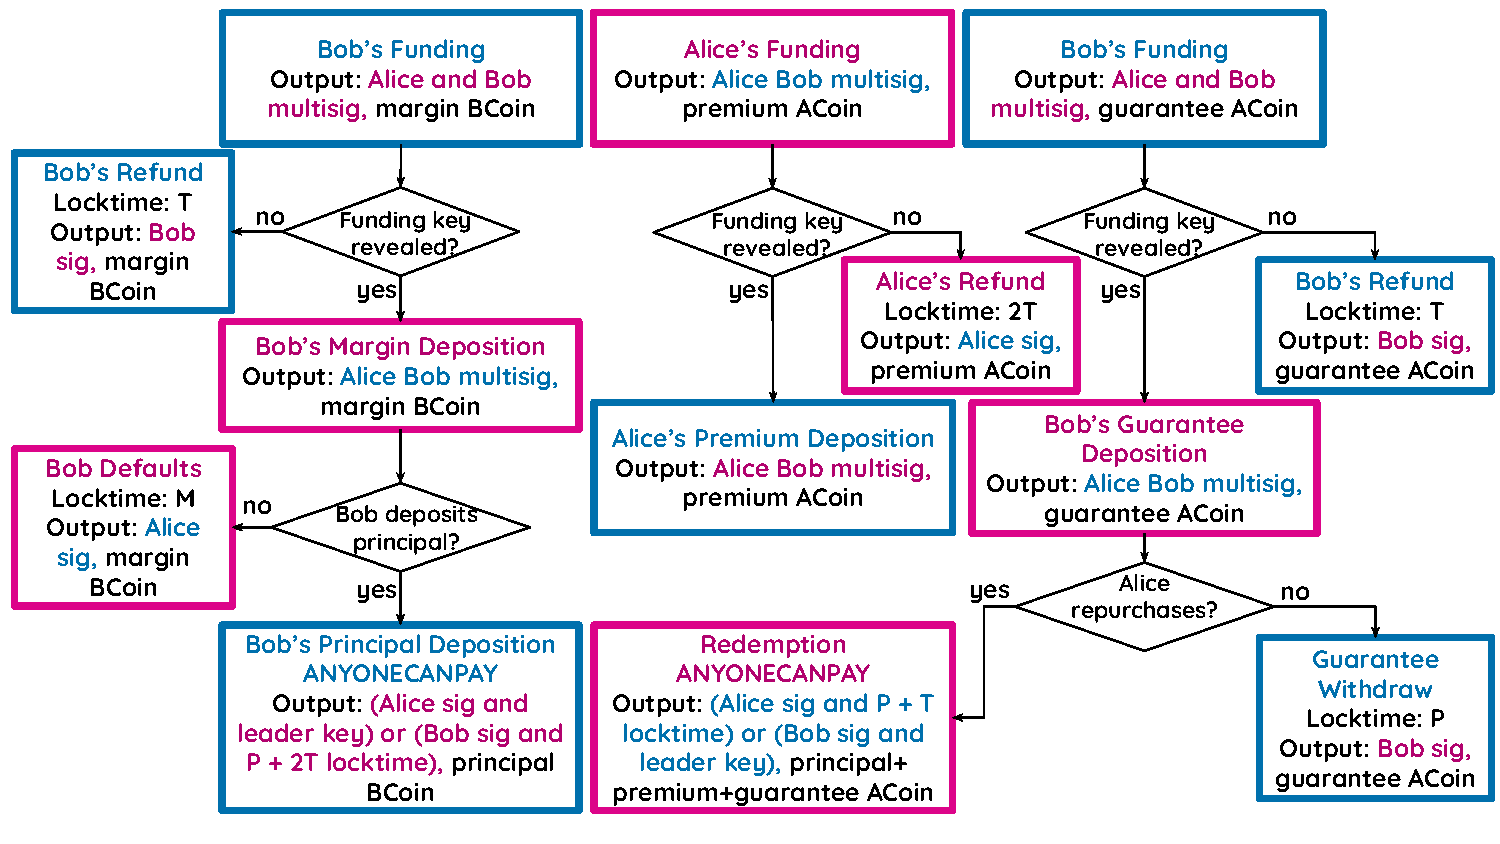
\includegraphics[width=0.5\textwidth]{ABCDfateme.pdf}
    \caption{ A flowchart for the protocol. All the transactions and their output scrips are shown. }
    \label{fig:flowchart}
\end{figure}
In this demo, Alice is the bond seller who borrows the principal and pays the premium, Bob is the bond buyer who lends the principal and gets the premium. Carol is the party with whom Alice makes another trade before paying Bob's principal back. Alice takes the principal from Bob in the Bitcoin testnet, performs an atomic swap with Carol between Bitcoin and Litecoin testnets, and pays Bob's principal back in Bitcoin. This is the normal way the protocol goes on. Of course, at any point, some coalition may decide to stop the procedure or intentionally deviate from the protocol in order to maximize their utility. The protocol supports situations where any set of parties behave abnormally. If Bob defaults, he will be punished by losing his margin. If either Alice or Carol defaults, Bob will gain the premium anyway. Finally, if Alice and Carol adhere to the protocol, and Bob avoids unlocking the principal, then Alice can punish Bob by acquiring Bob's guarantee amount. 


% \hfill mds
 
% \hfill August 26, 2015
\section{Transactions}
Fig.~\ref{fig:flowchart} shows the flow of the protocol and all the transactions. Transactions included in the ABCD are the followings:

\begin{figure}
    \centering
    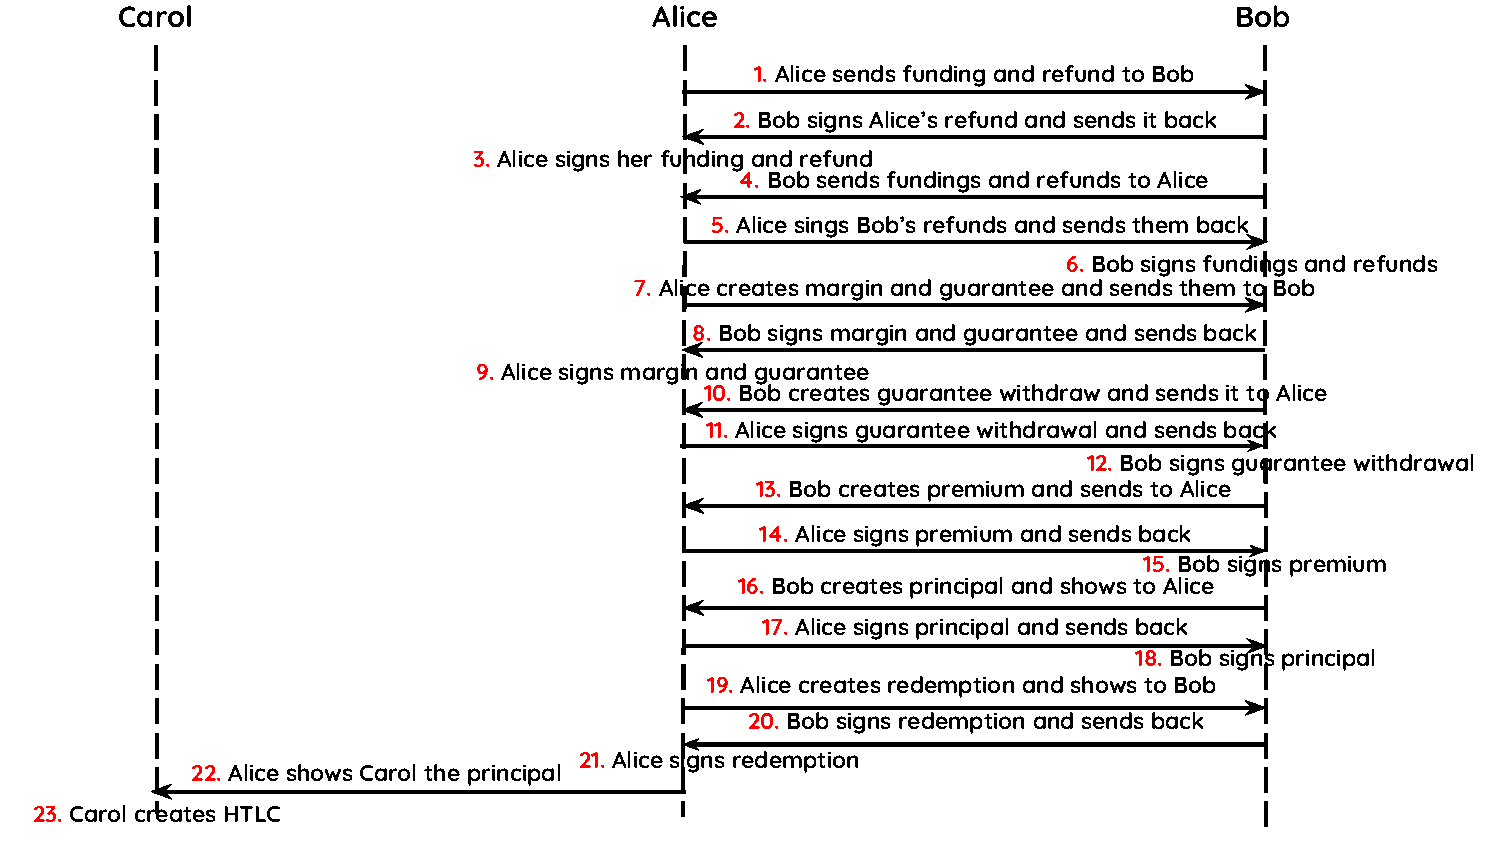
\includegraphics[width=0.5\textwidth]{ABCDinitializationn.pdf}
    \caption{Initialization phase}
    \label{fig:initialization}
\end{figure}
\begin{itemize}
    \item Funding: There are three funding transactions, one for Alice and two for Bob. In order to spend the funding transactions, either the \textit{funding key} has to be revealed or a certain amount of time has to be passed. The former represents the normal case, while the latter happens if Alice does not reveal the key.
    \item Refund: In case of any abnormal action from the other party, each party can use the refund to take the funding amount back.
    \item Margin Deposition and Guarantee Deposition: Using these transactions Alice moves Bob's fundings amount to the next step and also reveals the funding key. After confirming margin deposition and guarantee deposition transactions, Bob's refund transactions no longer work.
    %mention earlier that this is why Bob does the whole thing
    \item Premium Deposition: When Alice reveals the funding key, Bob broadcasts this transaction to pay the premium to himself and both parties go to the next stage.
    \item Redemption: This transaction is used for Alice to repurchase the bond. This is an any-one-can-pay transaction which means at the time of creating, not all the inputs need to be clear. Alice can later fulfill the transaction and pay her debt back. 
    \item Bob's Principal Deposition: Bob has to broadcast this transaction before $M$ locktime. By doing this, he is lending the principal to Alice. This transaction can not be spent without knowing the \textit{leader key}. So, Bob does not reveal it until Alice has broadcast the redemption transaction.
    % \item Alice Defaults: If Alice does not pay her debt back before $P$ locktime, Bob will broadcast this transaction and get his premium. He will never reveal the leader key so that Alice can not spend the bond.
    \item Bob Defaults: If Bob does not deposit the principal before $M$ locktime, Alice will take his margin as a punishment using this transaction.
    \item Guarantee Withdrawal: If Alice repurchases the bond within the expected time and Bob does not reveal the leader key, then Alice can punish Bob by spending the guarantee amount on the repurchase transaction to herself. Otherwise, Bob can pay the guarantee value back to himself using the guarantee withdrawal transaction.
\end{itemize}


\begin{figure}
\centering
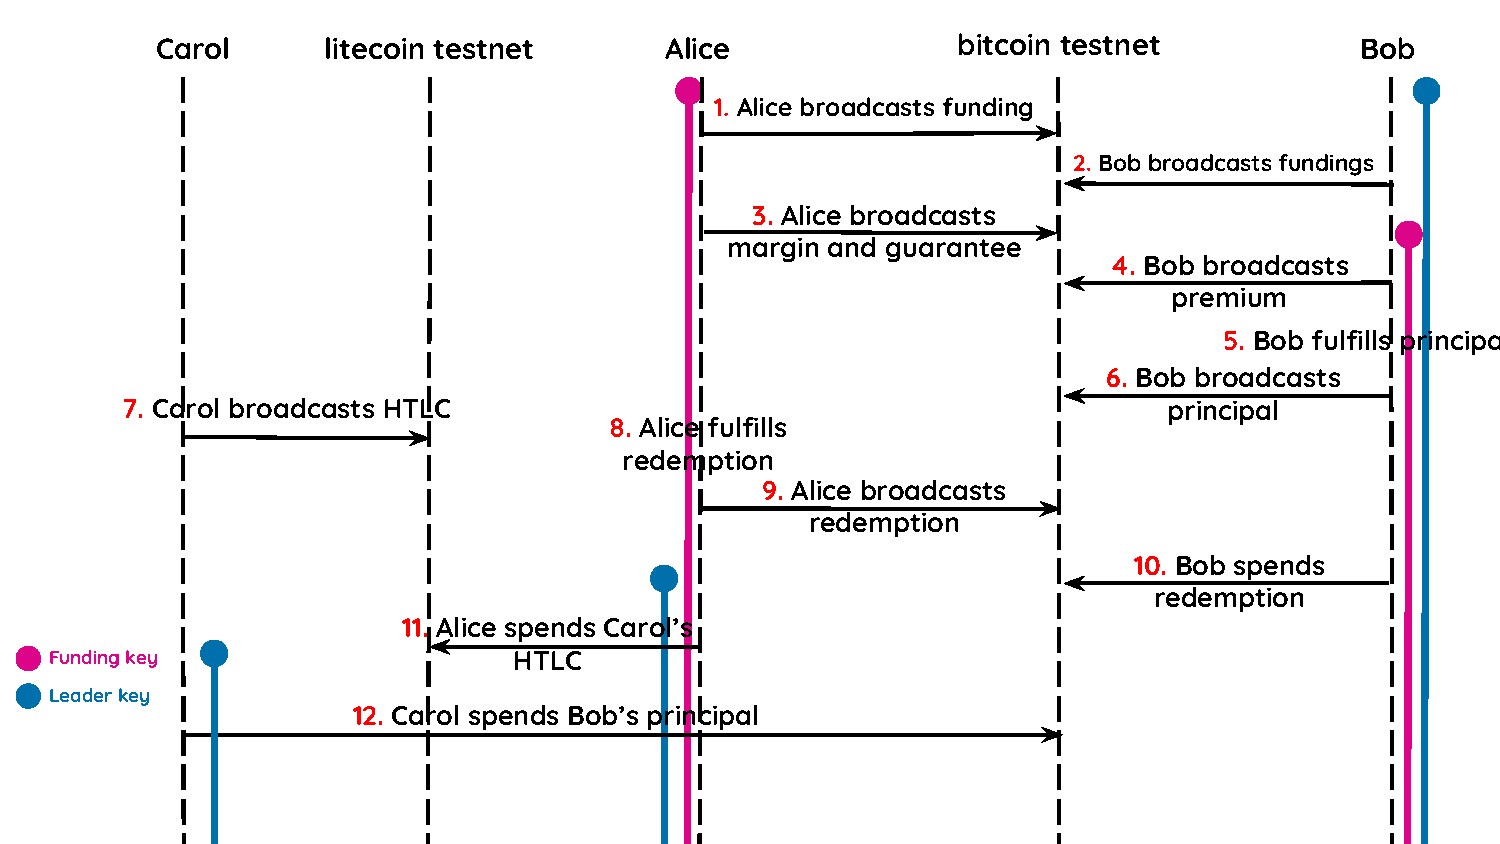
\includegraphics[width=0.5\textwidth]{ABCDarrows-3.pdf}
\caption{Commitment phase. Pink and blue bars indicate which party is aware of which secret and when.}
\label{fig:commitment}
\end{figure}
\section{Protocol}
The protocol of ABCD consists of two phases, initialization, and commitment.\\
\textbf{Initialization Phase}:
In this phase, the parties create transactions, exchange, and sign them. So, they make sure no one has the chance to cheat on the other. Fig.~\ref{fig:initialization} is an illustration of this phase. %Steps of this phase are:
% \begin{enumerate}
%     \item Alice creates the funding and refund transactions and sends them to Bob. Then, Bob signs the refund and sends it back to Alice. Now, Alice signs the funding and refund transactions. Bob does likewise to Alice. 
%     \item Alice creates the margin deposition and guarantee deposition transactions and sends them to Bob. Bob signs them and sends them back to Alice. Then Alice signs and keeps them. Bob does likewise for the guarantee withdrawal transaction and then for the premium and principal deposition transactions. Then, Alice does the same for the redemption transaction.
%     \item Finally, Alice shows the principal deposition transaction to Carol. Then, Carol creates an HTLC between herself and Bob.
% \end{enumerate}


\textbf{Commitment Phase:}
In this phase, they broadcast the transactions created in the previous phase dependent on whether they wish to abort everything or continue normally. Fig.~\ref{fig:commitment} shows the steps of this phase in the case that no one defaults.
Abnormal cases can occur in cases such as:
\begin{enumerate*}
    \item Alice does not broadcast her funding.
    \item Alice broadcasts the refund instead of margin and Bob would do likewise.
    \item Bob does not deposit the principal before the $M$ locktime, so Alice broadcasting the Bob defaults transaction would take his margin.
    \item Alice does not fulfill the redemption before the $P$ locktime, then Bob would take his margin and guarantee back, and he would not reveal the leader key.
\end{enumerate*}

  




% \begin{enumerate}
%     \item Alice broadcasts the funding transaction. If she was willing to abolish the whole procedure, she would not broadcast the funding.
    % \item Bob broadcasts his own fundings.
    % \item Alice broadcasts the margin deposition and guarantee deposition transactions and reveals the funding key, so the funding key reveals to Bob. In the abnormal case, she would broadcast the refund and Bob would do likewise.
    % \item Bob broadcasts the premium deposition transaction. If he does not, Alice will broadcast the refund. 
    %change the figure three
    % \item Bob fulfills the principal deposition transaction and broadcasts it.  %define default
    
    % \item When Carol sees the principal deposition transaction, she broadcasts her HTLC. %If she does not, Alice defaults as well. % what happens exactly?
    % \item Alice fulfills the redemption and broadcasts it. If she 
    % \item Bob spends the redemption. Doing this, he reveals the leader key.
    % \item Now, Alice knows the leader key. Thus, she spends Carol's HTLC.
    % \item Carol who now knows the leader key, spends Bob's principal and the procedure is over.
% \end{enumerate}



% \subsection{Subsection Heading Here}
% Subsection text here.


% \subsubsection{Subsubsection Heading Here}
% Subsubsection text here.


% An example of a floating figure using the graphicx package.
% Note that \label must occur AFTER (or within) \caption.
% For figures, \caption should occur after the \includegraphics.
% Note that IEEEtran v1.7 and later has special internal code that
% is designed to preserve the operation of \label within \caption
% even when the captionsoff option is in effect. However, because
% of issues like this, it may be the safest practice to put all your
% \label just after \caption rather than within \caption{}.
%
% Reminder: the "draftcls" or "draftclsnofoot", not "draft", class
% option should be used if it is desired that the figures are to be
% displayed while in draft mode.
%
%\begin{figure}[!t]
%\centering
%\includegraphics[width=2.5in]{myfigure}
% where an .eps filename suffix will be assumed under latex, 
% and a .pdf suffix will be assumed for pdflatex; or what has been declared
% via \DeclareGraphicsExtensions.
%\caption{Simulation results for the network.}
%\label{fig_sim}
%\end{figure}

% Note that the IEEE typically puts floats only at the top, even when this
% results in a large percentage of a column being occupied by floats.


% An example of a double column floating figure using two subfigures.
% (The subfig.sty package must be loaded for this to work.)
% The subfigure \label commands are set within each subfloat command,
% and the \label for the overall figure must come after \caption.
% \hfil is used as a separator to get equal spacing.
% Watch out that the combined width of all the subfigures on a 
% line do not exceed the text width or a line break will occur.
%
%\begin{figure*}[!t]
%\centering
%\subfloat[Case I]{\includegraphics[width=2.5in]{box}%
%\label{fig_first_case}}
%\hfil
%\subfloat[Case II]{\includegraphics[width=2.5in]{box}%
%\label{fig_second_case}}
%\caption{Simulation results for the network.}
%\label{fig_sim}
%\end{figure*}
%
% Note that often IEEE papers with subfigures do not employ subfigure
% captions (using the optional argument to \subfloat[]), but instead will
% reference/describe all of them (a), (b), etc., within the main caption.
% Be aware that for subfig.sty to generate the (a), (b), etc., subfigure
% labels, the optional argument to \subfloat must be present. If a
% subcaption is not desired, just leave its contents blank,
% e.g., \subfloat[].


% An example of a floating table. Note that, for IEEE style tables, the
% \caption command should come BEFORE the table and, given that table
% captions serve much like titles, are usually capitalized except for words
% such as a, an, and, as, at, but, by, for, in, nor, of, on, or, the, to
% and up, which are usually not capitalized unless they are the first or
% last word of the caption. Table text will default to \footnotesize as
% the IEEE normally uses this smaller font for tables.
% The \label must come after \caption as always.
%
%\begin{table}[!t]
%% increase table row spacing, adjust to taste
%\renewcommand{\arraystretch}{1.3}
% if using array.sty, it might be a good idea to tweak the value of
% \extrarowheight as needed to properly center the text within the cells
%\caption{An Example of a Table}
%\label{table_example}
%\centering
%% Some packages, such as MDW tools, offer better commands for making tables
%% than the plain LaTeX2e tabular which is used here.
%\begin{tabular}{|c||c|}
%\hline
%One & Two\\
%\hline
%Three & Four\\
%\hline
%\end{tabular}
%\end{table}


% Note that the IEEE does not put floats in the very first column
% - or typically anywhere on the first page for that matter. Also,
% in-text middle ("here") positioning is typically not used, but it
% is allowed and encouraged for Computer Society conferences (but
% not Computer Society journals). Most IEEE journals/conferences use
% top floats exclusively. 
% Note that, LaTeX2e, unlike IEEE journals/conferences, places
% footnotes above bottom floats. This can be corrected via the
% \fnbelowfloat command of the stfloats package.



\section{Conclusion}

In this article, we run an instance of ABCD on Bitcoin testnet and perform a simple atomic swap with the debt and Litecoin testnet tokens. The reference to the implementation of different scenarios of ABCD is accessible in ABCD official github page \href{https://github.com/incentivus/abcd}{https://github.com/incentivus/abcd}.


% conference papers do not normally have an appendix






% trigger a \newpage just before the given reference
% number - used to balance the columns on the last page
% adjust value as needed - may need to be readjusted if
% the document is modified later
%\IEEEtriggeratref{8}
% The "triggered" command can be changed if desired:
%\IEEEtriggercmd{\enlargethispage{-5in}}

% references section

% can use a bibliography generated by BibTeX as a .bbl file
% BibTeX documentation can be easily obtained at:
% http://mirror.ctan.org/biblio/bibtex/contrib/doc/
% The IEEEtran BibTeX style support page is at:
% http://www.michaelshell.org/tex/ieeetran/bibtex/
% \bibliographystyle{IEEEtran}
% argument is your BibTeX string definitions and bibliography database(s)
\bibliography{references}
\bibliographystyle{ieeetr}

%
% <OR> manually copy in the resultant .bbl file
% set second argument of \begin to the number of references
% (used to reserve space for the reference number labels box)
% \begin{thebibliography}{1}

% \bibitem{IEEEhowto:kopka}
% H.~Kopka and P.~W. Daly, \emph{A Guide to \LaTeX}, 3rd~ed.\hskip 1em plus
%   0.5em minus 0.4em\relax Harlow, England: Addison-Wesley, 1999.



% \end{thebibliography}



% that's all folks
\end{document}
